\section{Группы}
\begin{definition}
	Группа это множество с бинарной операцией для которой выполняются следующие свойства: 
	\begin{enumerate}
		\item Ассоциативность
		\item Наличие нейтрального элемента
		\item Наличие для каждого элемента обратного
	\end{enumerate}
	Если операция коммутативна, то группу также называют абелевой.
\end{definition}

\begin{definition}
	$f: G_1 \to G_2$ называется гомоморфизмом, если $\forall g, \widetilde{g} \ f(g \cdot \widetilde{g}) = f(g) \cdot f(\widetilde{g})$
\end{definition}

\begin{prop}
	$f(e) = e$
	\begin{proof}
		$f(e) = f(e \cdot e) = f(e) \cdot f(e)$, домножим на $(f(e))^{-1}$ с обеих сторон, тогда: $$e = f(e)$$
	\end{proof}
\end{prop}

\begin{examplelist}
	\item Циклическая группа $G = \{e, \gamma, \gamma^2, \dots, \}$
	\item $V$ - векторное конечномерное пространство, тогда $G = Aut\ V$ с композицей в качестве бинарной операции. Также такую группу называют $GL(V)$ - общей линейной группой (General Linear). Для матриц: $GL_n(k)$ - все матрицы $n \times n$ с ненулевым определителем над полем $k$.
	\item Если фиксировать базис $e_1, \dots, e_n$, то $L \in GL(V)$ можно представить в виде матрицы с ненулевым определителем. Тогда автоморфизмы из $GL(V)$ с определителем 1 образуют подгруппу $SL(V)$ - специальную линейную группу (Special Linear). Можно сказать, что такие автоморфизмы сохраняют объем. Для матриц: $SL_n(k)$ - все матрицы $n \times n$ с определителем 1 над полем $k$.
	\item В евклидовом пространстве рассмотрим автоморфизмы $f$, которые сохраняют длины: $$||f(v)|| = ||v|| \ \forall v \in V$$ Все такие $f$ образуют $O(V)$ - ортогональную группу. Для матриц: $O_n$ - ортогональные матрицы $n \times n$.
\end{examplelist}

\begin{example}
	Мы хотим посчитать $|GL(V)|$, где $V = \mathbb{F}_p^n$: зафиксируем базис $e_1, \dots, e_n$, $L \in GL(V)$. Теперь нам достаточно решить куда отправить базисные векторы. \\
	$L(e_1)$ - можем отправить куда угодно, кроме нуля - $\left(p^n - 1\right)$ вариантов. \\
	$L(e_2)$ - можем отправить куда угодно, кроме нуля и векторов коллинеарных $L(e_1)$ - $\left(p^n - n\right)$ вариантов. \\
	Тогда для $L(e_n)$ останется $\left(p^n - p^{n-1}\right)$ вариантов.
	$$|GL(V)| = \left(p - 1\right)\left(p^n - p\right)\dots\left(p^n - p^{n-1}\right)$$
\end{example}

\begin{definition}
	(Группа перестановок) \\ $X$ - множество, $G = S_X = \{f: X \to X: f - \text{биекция}\}$.\\ Если $X = \{1, \dots, n\}$, то $S_X = S_n$, $|S_n| = n!$
\end{definition}

\begin{definition}
	$\sigma \in S_n$ - перестановка, которую можно записать следующим образом:
	\[
		\begin{pmatrix}
			1 & 2 & \cdots & n \\
			\sigma(1) & \sigma(2) & \cdots & \sigma(n)
		\end{pmatrix}
	\]
	Дальше мы научимся удобнее записывать перестановки.
\end{definition}

\begin{definition}
	Перестановка $\sigma$, Которая циклически переставляет некоторые элементы из $X$, а остальные оставляет на месте, называется циклом.
	\[
	i_1 \overset{\sigma}{\mapsto} i_2 \overset{\sigma}{\mapsto} i_3 \overset{\sigma}{\mapsto} i_1
	\]
\end{definition}

\begin{stmt}
	$\forall \sigma \in S_n$ раскладывается в произведение циклов единственным образом с точностью до порядка циклов.
	\begin{proof}
		Выберем $x \in X = \{1, \dots, n\}$ и рассмотрим $Y \subset X = \{x, \sigma x, \sigma^2 x, \dots\}$
		\[
		\sigma_1(y) = 
		\begin{cases}
			y, y \notin Y \\
			\sigma(y), y \in Y
		\end{cases} \text{ -- биекция}
		\]
		Мы можем делать так для всех элементов из $X$, которые не вошли в $Y$. \\ Например, возьмем $z \notin Y$, $Z = \{z, \sigma z, \sigma^2 z, \dots\}$ \\
		Заметим, что $Y \cap Z = \varnothing$, иначе, если $\exists \alpha \in Y \cap Z$, то $\alpha = \sigma^k x$, $\alpha = \sigma^m z$ с минимальными выбранными $k$ и $m$. \\
		Тогда $\sigma(\sigma^{k-1}x) = \alpha$ и $\sigma(\sigma^{m-1}z) = \alpha$, что нарушает биекцию. 
		\[
		\sigma = \sigma_1 \sigma_2 \dots \sigma_t
		\]
	\end{proof}
\end{stmt}

\begin{example}
	\[
	\sigma = \begin{pmatrix}
		1 & 2 & 3 & 4 & 5 & 6 & 7 \\
		3 & 2 & 1 & 5 & 6 & 7 & 4
	\end{pmatrix}
	\]
	$$\sigma = (1 \to 3) (2) (4 \to 5 \to 6 \to 7) = (13)(4567)$$
\end{example}

\begin{definition}(Группа диэдра) \\
	$X$ - правильный $n$-угольник на плоскости с центром в 0 \\
	$D_n$ - группа элементов из $O\left(\mathbb{R}^2\right)$, переводящие $X$ в себя, такую группу называют группой диэдра.
\end{definition}

\begin{examplelist}
	\item $n = 2$ \\
	В данном случае наша фигура выглядит следующим образом:
	\begin{center}
		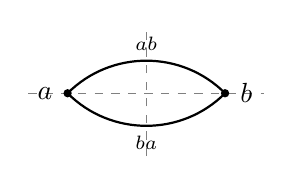
\begin{tikzpicture}[
			lens/.style={
				draw, thick,
				bend left=45
			},
			label node/.style={font=\scriptsize},
			axis/.style={dashed, gray, thin}
			]
			\coordinate (v1l) at (0,0) {};
			\coordinate (v1r) at (2,0) {};
			
			\draw[axis] (-0.5, 0) -- (2.5, 0);
			\draw[axis] (1, -0.8) -- (1, 0.8);
			
			\draw [lens] (v1l.center) to node[above, label node] {$ab$} (v1r.center);
			\draw [lens] (v1r.center) to node[below, label node] {$ba$} (v1l.center);
			
			\fill (v1l) circle (1.5pt);
			\fill (v1r) circle (1.5pt);
			
			\node[left=2pt] at (v1l) {$a$};
			\node[right=2pt] at (v1r) {$b$};
			
		\end{tikzpicture}
	\end{center}
	Пусть $\tau$ - поворот фигуры на $\pi$, $\varepsilon$ - отражение относительно вертикальной оси, $\widetilde{\varepsilon}$ - отражение относительно горизонтальной оси. Тогда $D_2 = \{e, \tau, \varepsilon, \widetilde{\varepsilon}\}$. \\
	Распишем $\tau \varepsilon$: \\
	\begin{center}
		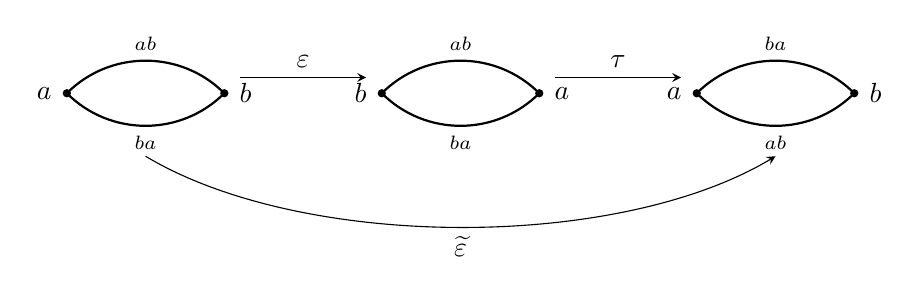
\begin{tikzpicture}[
			>=stealth,
			lens/.style={
				draw, thick,
				bend left = 45
			},
			label node/.style={font=\scriptsize}
			]
			\coordinate (v1l) at (0,0) {};
			\coordinate (v1r) at (2,0) {};
			\draw [lens] (v1l.center) to node[above, label node] {$ab$} (v1r.center);
			\draw [lens] (v1r.center) to node[below, label node] {$ba$} (v1l.center);
			
			\fill (v1l) circle (1.5pt);
			\fill (v1r) circle (1.5pt);
			
			\node[left=2pt] at (v1l) {$a$};
			\node[right=2pt] at (v1r) {$b$};
			
			\begin{scope}[xshift=4cm]
				\coordinate (v2l) at (0,0) {};
				\coordinate (v2r) at (2,0) {};
				\draw [lens] (v2l.center) to node[above, label node] {$ab$} (v2r.center);
				\draw [lens] (v2r.center) to node[below, label node] {$ba$} (v2l.center);
				\fill (v2l) circle (1.5pt);
				\fill (v2r) circle (1.5pt);
				\node[left=2pt] at (v2l) {$b$};
				\node[right=2pt] at (v2r) {$a$};
			\end{scope}
			
			\begin{scope}[xshift=8cm]
				\coordinate (v3l) at (0,0) {};
				\coordinate (v3r) at (2,0) {};
				\draw [lens] (v3l.center) to node[above, label node] {$ba$} (v3r.center);
				\draw [lens] (v3r.center) to node[below, label node] {$ab$} (v3l.center);
				\fill (v3l) circle (1.5pt);
				\fill (v3r) circle (1.5pt);
				\node[left=2pt] at (v3l) {$a$};
				\node[right=2pt] at (v3r) {$b$};
			\end{scope}
			
			\draw[->] (2.2, 0.2) -- node[above] {$\varepsilon$} (3.8, 0.2);
			\draw[->] (6.2, 0.2) -- node[above] {$\tau$} (7.8, 0.2);
			\draw[->] (1, -0.8) .. controls (3, -2) and (7, -2) .. node[below] {$\widetilde{\varepsilon}$} (9, -0.8);
			
			
		\end{tikzpicture}
	\end{center}
	Заметим, что $\widetilde{\varepsilon} = \tau \varepsilon$, тогда $D_2 = \{e, \tau, \varepsilon, \tau \varepsilon\}$. У нас четыре элемента порядка два, поэтому $$D_2 \overset{\sim}{=} \mathbb{Z}/2\mathbb{Z} \oplus \mathbb{Z}/2\mathbb{Z}.$$
	\item $n = 3$ \\
	В данном случае наша фигура выглядит следующим образом:
	\begin{center}
		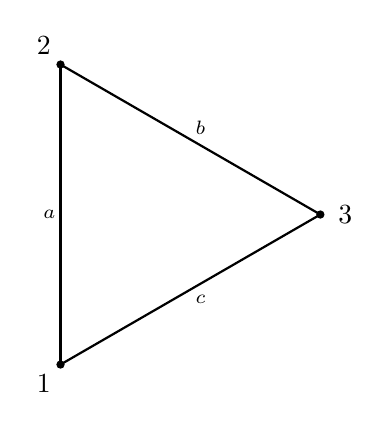
\begin{tikzpicture}[
			label node/.style={font=\scriptsize, inner sep=1.5pt},
			axis dashed/.style={dashed, gray, thin}
			]
			\def\R{2.2cm}
			\coordinate (V2) at (120:\R);
			\coordinate (V1) at (240:\R);
			\coordinate (V3) at (0:\R);
			\draw[thick] (V1) -- node[left, label node] {$a$} (V2);
			\draw[thick] (V2) -- node[above right, label node] {$b$} (V3);
			\draw[thick] (V3) -- node[below right, label node] {$c$} (V1);
			
			\fill (V1) circle (1.5pt) node[below left] {1};
			\fill (V2) circle (1.5pt) node[above left] {2};
			\fill (V3) circle (1.5pt) node[right=3pt] {3};
		\end{tikzpicture}
	\end{center}
	Пусть $\tau$ - поворот на $\frac{2\pi}{3}$, $\varepsilon$ - отражение по горизонтали, тогда $D_3 = \{e, \tau, \tau^2, \varepsilon, \varepsilon\tau, \varepsilon\tau^2\}$\\
	Распишем $\tau \varepsilon$
	\begin{center}
		\begin{tikzpicture}[
			>=stealth,
			tri line/.style={thick},
			label node/.style={font=\scriptsize},
			vertex node/.style={font=\scriptsize, inner sep=1pt}
			]
			\newcommand{\drawtri}[6]{
				\coordinate (V3) at (0:1.2);
				\coordinate (V2) at (120:1.2);
				\coordinate (V1) at (240:1.2);
				
				\draw[tri line] (V1) -- node[left, label node] {#4} (V2);
				\draw[tri line] (V2) -- node[above right, label node] {#5} (V3);
				\draw[tri line] (V3) -- node[below right, label node] {#6} (V1);
				
				\node[above, vertex node] at (V2) {#1};
				\node[below, vertex node] at (V1) {#2};
				\node[right, vertex node] at (V3) {#3};
			}
			\begin{scope}[xshift=0cm]
				\drawtri{2}{1}{3}{a}{b}{c}
				\coordinate (StartArrow) at (0,-1.3);
			\end{scope}
			\draw[->] (1.5, 0) -- node[above] {$\varepsilon$} (2.3, 0);
			\begin{scope}[xshift=3.5cm]
				\drawtri{1}{2}{3}{a}{c}{b}
			\end{scope}
			\draw[->] (5, 0) -- node[above] {$\tau$} (5.8, 0);
			\begin{scope}[xshift=7cm]
				\drawtri{3}{1}{2}{c}{b}{a}
				\coordinate (EndArrow) at (0,-1.3); % Точка для длинной стрелки
			\end{scope}
			\draw[->, thick] (StartArrow) .. controls (1.5,-2.5) and (5.5,-2.5) .. node[below]{$\tau \varepsilon$} (EndArrow);
		\end{tikzpicture}
	\end{center}
	Распишем $\varepsilon \tau^2$: \\
	\begin{center}
		\begin{tikzpicture}[
			>=stealth,
			tri line/.style={thick},
			label node/.style={font=\scriptsize},
			vertex node/.style={font=\scriptsize, inner sep=1pt}
			]
			\newcommand{\drawtri}[6]{
				\coordinate (V3) at (0:1.2);
				\coordinate (V2) at (120:1.2);
				\coordinate (V1) at (240:1.2);
				
				\draw[tri line] (V1) -- node[left, label node] {#4} (V2);
				\draw[tri line] (V2) -- node[above right, label node] {#5} (V3);
				\draw[tri line] (V3) -- node[below right, label node] {#6} (V1);
				
				\node[above, vertex node] at (V2) {#1};
				\node[below, vertex node] at (V1) {#2};
				\node[right, vertex node] at (V3) {#3};
			}
			\begin{scope}[xshift=0cm]
				\drawtri{2}{1}{3}{a}{b}{c}
				\coordinate (StartArrow) at (0,-1.3);
			\end{scope}
			\draw[->] (1.5, 0) -- node[above] {$\tau^2$} (2.3, 0);
			\begin{scope}[xshift=3.5cm]
				\drawtri{1}{3}{2}{c}{a}{b}
			\end{scope}
			\draw[->] (5, 0) -- node[above] {$\tau$} (5.8, 0);
			\begin{scope}[xshift=7cm]
				\drawtri{3}{1}{2}{c}{a}{b}
				\coordinate (EndArrow) at (0,-1.3); % Точка для длинной стрелки
			\end{scope}
			\draw[->, thick] (StartArrow) .. controls (1.5,-2.5) and (5.5,-2.5) .. node[below]{$\tau \varepsilon$} (EndArrow);
		\end{tikzpicture}
	\end{center}
	Заметим, что $\varepsilon\tau^2 = \tau\varepsilon$. Любой элемент из $D_3$ можно описать перестановкой вершин, тогда: 
	\[
	D_3 \overset{\sim}{=} S_3
	\]
\end{examplelist}

\begin{definition}(Ядро) \\
	$G, H$ - группы, $\varphi: G \to H$ - гомоморфизм.
	\[
	\ker\varphi = \left\{g \in G: \varphi(g) = e\right\}
	\]
\end{definition}

\begin{stmt}
	Пусть $h, \widetilde{h} \in H$. Тогда $\exists$ биекция $\varphi^{-1}(h) \to \varphi^{-1}(\widetilde{h})$, если они не пусты.
	\begin{proof}
		покажем, что $\forall h \in \ Im\varphi$ существует биекция $\ker\varphi \to \varphi^{-1}(h)$ \\
		Пусть $g \in \varphi^{-1}(h)$ - фиксированный элемент, рассмотрим $\widetilde{g} \in \varphi^{-1}(h)$ \\
		Мы хотим, чтобы $gz = \widetilde{g} \implies z = g^{-1}\widetilde{g}$
		\[
		\varphi(z) = \varphi(g^{-1}\widetilde{g}) = \varphi(g)^{-1} \varphi(\widetilde{g}) = h^{-1}h = e
		\]
		С другой стороны, если $z \in \ker \varphi$, то $gz \in \varphi^{-1}(h)$\\
		Строим $\underset{z \mapsto gz}{\ker\varphi \to \varphi^{-1}(h)}$ - биекция
	\end{proof}
\end{stmt}

\begin{cor}
	Пусть $\varphi: G \to H$ - гомоморфизм групп, тогда 
	\[
	|Im\varphi| = \frac{|G|}{|\ker\varphi|}
	\]
\end{cor}

\begin{example}
	Посчитаем $|SL(\mathbb{F}_p^n)|$. Введем отображение $GL(\mathbb{F}_p^n) \overset{\det}{\to} \mathbb{F}_p^x$, где $\ker\left(\det\right) = SL(\mathbb{F}_p^n)$, тогда по следствию:
	\[
	|\mathbb{F}_p^x| = \frac{|GL(\mathbb{F}_p^n)|}{|SL(\mathbb{F}_p^n)|} \implies |SL(\mathbb{F}_p^n)| = \frac{(p^n - 1)\dots(p^n - p^{n-1})}{p-1}
	\]
\end{example}

\begin{definition} (Действие группы)
	$G$ - группа, $X$ - множество \\
	Действием группы $G$ на множестве $X$ называется гомоморфизм $G \to BijX$.
\end{definition}

\begin{definition} (Орбита)
	$x \in X, G$ - группа, действующая на $X$
	\[
	Orb\ x = \{\varphi_g(x): g \in G\}
	\]
\end{definition}

\begin{definition}(Стабилизатор)
	$x \in X, G$ - группа, действующая на $X$
	\[
	Stab\ x = \{g \in G: \varphi_g(x) = x\}
	\]
\end{definition}